\documentclass{beamer}
%
%
\mode<presentation>
{
  \usetheme{default}      % or try Darmstadt, Madrid, Warsaw, ...
  \usecolortheme{default} % or try albatross, beaver, crane, ...
  \usefonttheme{default}  % or try serif, structurebold, ...
  \setbeamertemplate{navigation symbols}{}
  \setbeamertemplate{caption}[numbered]
} 

\usepackage[english]{babel}
\usepackage[utf8x]{inputenc}
\usepackage{adjustbox}
\usepackage{comment}
%\usepackage{fancyvrb}
\usepackage{pgffor}
%\usepackage{multirow}
\usepackage{mathtools}
%\usepackage{pdflscape}
%\usepackage{pdfpages}

\usepackage{amsmath}
\newcommand{\btVFill}{\vskip0pt plus 1filll}

\usepackage{totcount}
\regtotcounter{section}

\usepackage{datetime}                           % custom date
        \newdateformat{mydate}{\monthname[\THEMONTH] \THEYEAR}

\title[Your Short Title]{Solving the phase boundary between two solid phases via the common tangent procedure}
\author{David C. de Busturia}
\institute{Department of Chemistry. Imperial College London}
%\date{Date of Presentation}
%\date{}

% Add name of section in footline - no format, just the name
%\makeatletter
%\setbeamertemplate{footline}{%
%\leavevmode
%\vbox{\begin{beamercolorbox}[dp=1.25ex,ht=2.75ex]{fg=black}%
%  \hspace*{1em}\insertsectionhead%
%  \ifx\insertsubsectionhead\@empty\relax\else$\quad\mid\quad$\insertsubsectionhead\fi
%  \end{beamercolorbox}%
%  }%
%}
%\makeatother

% For inserting python code:
\usepackage{listings}

\usepackage{color}

\definecolor{codegreen}{rgb}{0,0.6,0}
\definecolor{codegray}{rgb}{0.5,0.5,0.5}
\definecolor{codepurple}{rgb}{0.58,0,0.82}
\definecolor{backcolour}{rgb}{0.95,0.95,0.92}
 
\lstdefinestyle{mystyle}{
    backgroundcolor=\color{backcolour},   
    commentstyle=\color{codegreen},
    keywordstyle=\color{magenta},
    numberstyle=\tiny\color{codegray},
    stringstyle=\color{codepurple},
    basicstyle=\footnotesize,
    breakatwhitespace=false,         
    breaklines=true,                 
    captionpos=b,                    
    keepspaces=true,                 
    numbers=left,                    
    numbersep=5pt,                  
    showspaces=false,                
    showstringspaces=false,
    showtabs=false,                  
    tabsize=2
}
 
\lstset{style=mystyle}
\newcommand\Fontvi{\fontsize{6}{5.2}\selectfont}
\newcommand\Fontvii{\fontsize{4}{4.2}\selectfont}


\newcounter{prevsec}

% Outline at the beginning of every section:
\AtBeginSection[]{\label{sec:\thesection}
  \begin{frame}[allowframebreaks]{Outline}
       \tableofcontents[
         currentsection,
         sectionstyle=show/shaded,
         subsectionstyle=shaded/shaded/shaded,
         subsubsectionstyle=shaded/shaded/shaded/shaded
         ]
  \end{frame}
}

% Outline at the beginning of each subsection:
\AtBeginSubsection[]
{
    \begin{frame}[allowframebreaks]{Outline}
        \tableofcontents[currentsection,currentsubsection]
    \end{frame}
}

% Outline at the beginning of each subsubsection:
\AtBeginSubsubsection[]
{
    \begin{frame}[allowframebreaks]{Outline}
        \tableofcontents[currentsection,currentsubsection]
    \end{frame}
}

\date{\today} % Date for the report
%\date{}
%\mydate{\today}
%\date{\mydate}
%\date{\mydate\today}

% This allows to print in a printer in 1 pdf page in 1 page, If commented, you'll have a tiny zoomed of each page in the prited version. Unfortunately this destroys hyperliks. 
%\usepackage{pgfpages}
%\pgfpagesuselayout{resize to}[a4paper,border shrink=5mm,landscape]





\begin{document}


\def\folders{10.00K,
30.10K,
50.20K,
70.30K,
90.40K,
110.51K,
130.61K,
150.71K,
170.81K,
190.91K,
211.01K,
231.11K,
251.21K,
271.31K,
291.41K,
311.52K,
331.62K,
351.72K}
%371.82K,
%391.92K,
%412.02K,
%432.12K,
%452.22K,
%472.32K,
%492.42K,
%512.53K,
%532.63K,
%552.73K,
%572.83K,
%592.93K}

%613.03K
%633.13K
%653.23K
%673.33K
%693.43K
%713.54K
%733.64K
%753.74K
%773.84K
%793.94K
%814.04K
%834.14K
%854.24K
%874.34K
%894.44K
%914.55K
%934.65K
%954.75K
%974.85K
%994.95K
%1015.05K
%1035.15K
%1055.25K
%1075.35K
%1095.45K
%1115.56K
%1135.66K
%1155.76K
%1175.86K
%1195.96K
%1216.06K
%1236.16K
%1256.26K
%1276.36K
%1296.46K
%1316.57K
%1336.67K
%1356.77K
%1376.87K
%1396.97K
%1417.07K
%1437.17K
%1457.27K
%1477.37K
%1497.47K
%1517.58K
%1537.68K
%1557.78K
%1577.88K
%1597.98K
%1618.08K
%1638.18K
%1658.28K
%1678.38K
%1698.48K
%1718.59K
%1738.69K
%1758.79K
%1778.89K
%1798.99K
%1819.09K
%1839.19K
%1859.29K
%1879.39K
%1899.49K
%1919.60K
%1939.70K
%1959.80K
%1979.90K
%2000.00K
%"


\newcommand{\Funkytable}[1]{
$T = {#1}$
%\begin{table}
%\centering
%\begin{adjustbox}{width={\textwidth},totalheight={\textheight},keepaspectratio}%
%\begin{tabular}{c|c|c|c|c}
%$F = E+E_{\mathit{ZP}} + \mathit{ET} - \mathit{TS}$ & $V$ & $P= -\frac{\partial (E+E_{\mathit{ZP}} + \mathit{ET} - \mathit{TS}) }{\partial V}$ & $G = E + E_{\mathit{ZP}} + \mathit{ET} - \mathit{TS}  + PV$ & $G^{I}$ and $G^{II}$ at {#1}\\\hline
%$\cdots$ & $\cdots$ & $\cdots$ & $\cdots$ & Interpolation %@ 10.00K
%\end{tabular}
%\end{adjustbox}
%\end{table}
}

%\maketitle % Insert the title, author and date

\defverbatim[colored]\lst{%
\begin{lstlisting}[tabsize=8,basicstyle=\ttfamily]
const char *processing() const{
    somestring = "-1";
}
\end{lstlisting}
}

\begin{frame}
  \titlepage
\end{frame}

% Uncomment these lines for an automatically generated outline.
\begin{frame}{Outline}
  \tableofcontents
\end{frame}



\section{$E(V)$, $E(V) + E_{ZP}$, $F(V; T)$ and pressure of transition. Thermal evolution}

\begin{frame}
\makebox[\textwidth]{%
\begin{minipage}{1.05\textwidth} % <--- can be as large the slide size permits
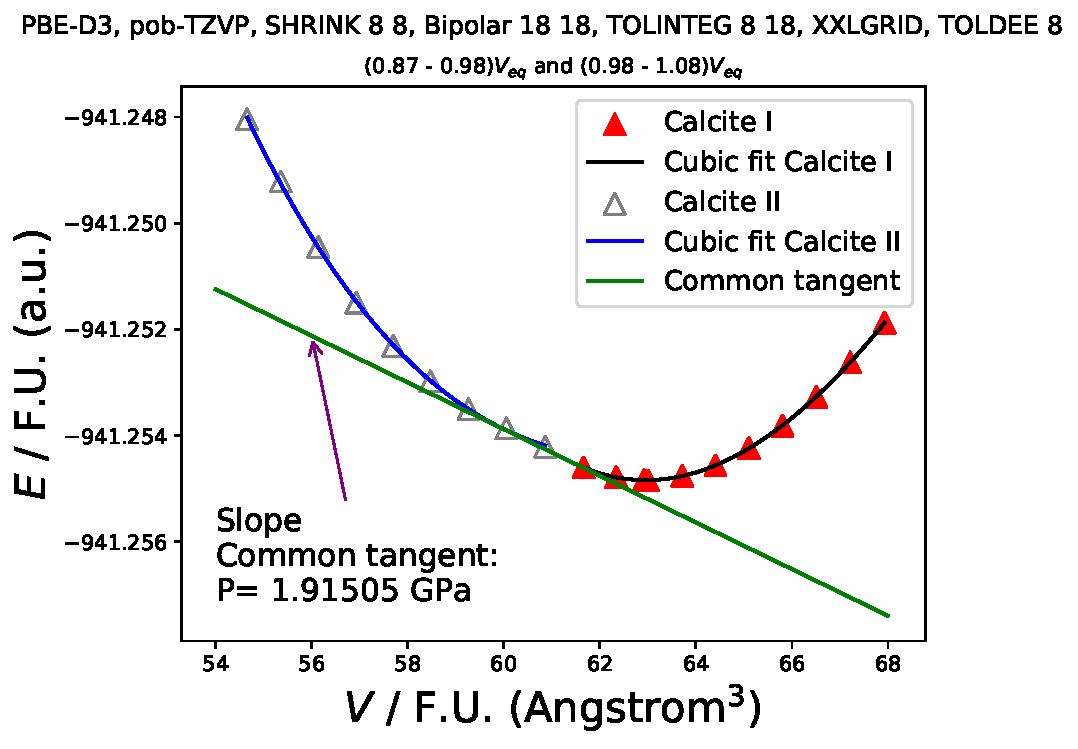
\includegraphics[width=.49\textwidth,keepaspectratio]{./EL_level/calcite_I_and_II_all_2_summary_better_plot.pdf}\hfill%
\end{minipage}
}

\end{frame}


\begin{frame}
\makebox[\textwidth]{%
\begin{minipage}{1.05\textwidth} % <--- can be as large the slide size permits
\includegraphics[width=.49\textwidth,keepaspectratio]{./EL_plus_E0_level/calcite_I_and_II_all_2_summary_better_plot.pdf}\hfill%
\end{minipage}
}

\end{frame}

\begin{frame}%{Main results}
\vspace{-1em}
\foreach \X [count=\Y]in \folders
{
\only<\Y>{
\Funkytable{\X}
}
\only<\Y>{
%\vspace{-3em}
\makebox[\textwidth]{
\begin{minipage}{1.05\textwidth} %
\includegraphics[width=.49\textwidth,keepaspectratio]{./G_PT/\X/calcite_I_and_II_all_2_summary_better_plot.pdf}\hfill%
\end{minipage}%
} %
}
%\pause
}
\end{frame}


\section{Phase Boundary}

\begin{frame}
\begin{figure}
\centering
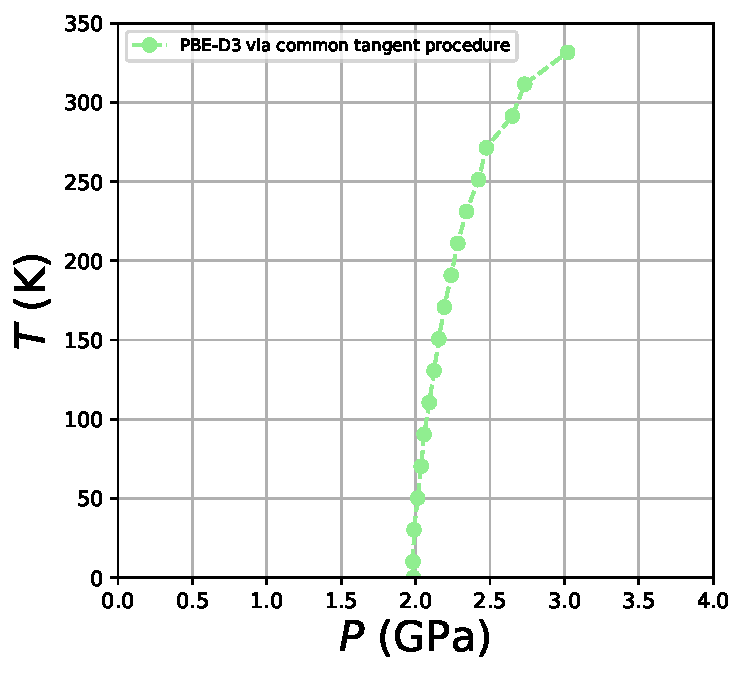
\includegraphics[width=.70\textwidth,keepaspectratio]{./calcite_I_and_II_phase_boundary.pdf}
\vspace{-1em}
\caption{Pressure-temperature phase boundary}
\end{figure}


\end{frame}

\end{document}

